\section{Simulations}

\subsection{Rotational cooling}

\todo{TBD}

\subsection{Non-adiabatic transitions}

Molecules travelling from the first state preparation region into the electrostatic lens experience fast changes in external electric field. Due to the large number of hyperfine levels involved, predicting level stability is a non-trivial task. As a consequence of the von Neumann--Wigner rule \cite{mead1979noncrossing}, levels of same symmetry will in general avoid crossing each other. Considering only a single such avoided crossing between a pair of states, we may model the situation using the two-level Hamiltonian
%
\begin{align}
    \label{twostate}
    H=\begin{pmatrix}
        \delta-\alpha\epsilon^2&\beta\\
        \beta&0
    \end{pmatrix},
\end{align}
%
where $\delta\propto2\pi\times100\kHz$ is the field-free level separation, $\alpha\epsilon^2$ is the level shift due to a quadratic Stark effect; thus $\alpha$ sets the field at which the Stark effect cancels $\delta$ (typically, tens or hundreds of V/cm). Finally, $\beta$ is the level coupling that gives rise to the avoided crossing. \todo{Define $\epsilon$. A plot would help.}

The Hamiltonian $H$ may be diagonalized exactly to give the eigenenergies $E_\pm$ and states $\psi_\pm$. To investigate the effect of subjecting the molecule to a time-varying electric field $\epsilon(t)$, we can assume that at $t=0$ the system starts in the state $\psi_+$. After solving the time-dependent Schr\"odinger equation (\TDSE) $id\psi/dt=H\psi$ for the final state $\psi_\text{f}$, we can evaluate the probability $P_\text{trans}=|\braket{\psi_\text{f}}{\psi_-}|^2$ the system has transitioned to the other field-free eigenstate.

If the electric field is chosen such that the system is taken through the avoided crossing in a time $T_\text{fall}$, then the transition probability $P_\text{trans}(T_\text{fall})$ approaches zero in both limits $T_\text{fall}\to0$ and $T_\text{fall}\to\infty$ (see Fig.~\ref{floquet}a). For intermediate times, the system exhibits a pattern of interference fringes, with $P_\text{trans}$ very sensitive to the exact timing of the electric field changes. For a molecular beam entering the electrostatic lens with a range of velocities, an initial hyperfine level could end up in a range of final states, preventing and defeating the focusing otherwise expected of the lens. \todo{you need more background/explanation of what is going on here \&\ why it is important to us}

\begin{figure}
    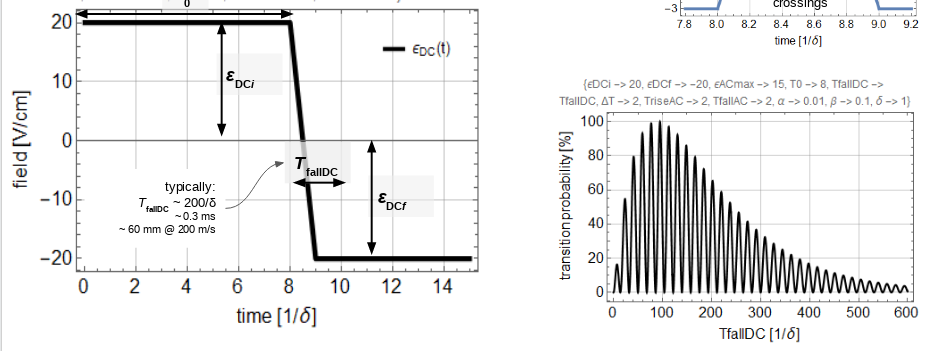
\includegraphics[width=.5\textwidth]{figs/floquet1.png}
    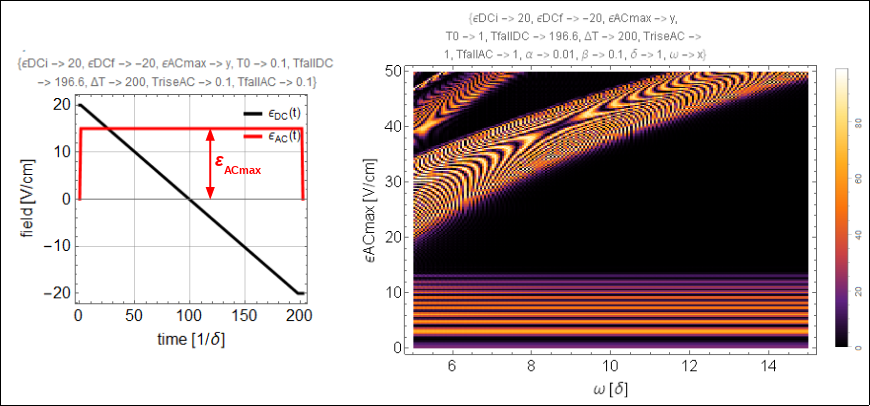
\includegraphics[width=.5\textwidth]{figs/floquet2.png}
    \caption{AC level stabilization against non-adiabtic transitions when subjected to time-varying electric fields. \part{Top} The transition-probability interference fringes as a function of field reversal time. \part{Bottom} Adding an \AC\ field results in separated regions of high $P_\text{trans}$ against a transition-free background. \todo{TODO: Make the labels readable! should also show instantaneous energy levels vs time.}}
    \label{floquet}
\end{figure}

Adding to the above a rapidly-oscillating \AC\ electric field can under certain conditions suppress the transitions otherwise expected in the absence of the \AC\ field. A plot of $P_\text{trans}$ with respect to the parameters of the \AC\ field (Fig.~\ref{floquet}b) shows separated regions of high $P_\text{trans}$ against a transition-free background. Furthermore, one of the regions does not show dependence on the frequency $\omega$ of the oscillating field, while the other regions show what appears to be polynomial dependence on $\omega$.

The above results can be qualitatively be interpreted in terms of Floquet theory for `stationary' states of periodically driven systems \cite[ch.~5]{dittrich1998quantum}. It can be proven that the \TDSE\ of such a system has solutions of form \cite[sect.~II.A]{shirley1965solution}
%
\[
\exp(-i\epsilon_\alpha t\hbar)\Phi_\alpha(x,t),
\]
%
where the periodic Floquet modes $\Phi_\alpha(x,t)$ satisfy a `time-independent' Schr\"odinger equation (\TISE) in extended Hilbert space $L_2[0,T]\otimes H$
%
\[
\underbrace{\left[H(t)-i\hbar\frac{\partial}{\partial t}\right]}_{\widetilde{H}}\Phi_\alpha(t)=\epsilon_\alpha\Phi_\alpha(t),
\]
%
To obtain the matrix elements of the Hamiltonian thus modified, we expand the Floquet modes in a basis $\{\ket{k}\}$ of $H$, and also in terms of $n$th order plane waves $e^{in\omega t}$:
%
\[
\Phi_\alpha(t)=\sum\limits_k\sum\limits_{n=-\infty}^\infty c_\alpha^{kn}e^{in\omega t}\ket{k}.
\]
%
Insert into the \TISE, pre-multiply by $\bra{j}e^{-im\omega t}$, and time-average over one cycle to obtain
%
\[
\sum\limits_{kn}\bra{j}\widetilde{H}\ket{k}c_\alpha^{kn}=\epsilon_\alpha c_\alpha^{jm},
\]
%
where the matrix elements of the extended Hamiltonian $\widetilde{H}$ are given in terms of the original Hamiltonian split into constant and time-varying parts $H(t)\equiv H_\text{DC}+H_\text{AC}(t)$:
%
\begin{align*}
    \label{floqMatElems}
    \widetilde{H}_{nm}^{jk}&=
    H_\text{DC}^{jk}\delta_{nm}
    +n\hbar\omega\delta_{nm}\delta^{jk}
    &\text{(atom + light)}\\
    &+\frac{1}{T}\int\limits_0^TH_\text{AC}^{jk}(t)e^{i(n-m)\omega t}dt.
    &\text{(interaction)}
\end{align*}
%
Here, the lower indices refer to a particular `photonic' mode, and the upper indices refer to the matrix elements of the original Hamiltonian.

The interaction term in the above general expression can easily be found for the case of the two-level model in eqn~\ref{twostate}. When an electric field $\epsilon(t)\equiv\epsilon_\text{DC}+\epsilon_\text{AC}(t)$ is applied, the \AC\ part of the Hamiltonian is
%
\[
H_\text{AC}=-\begin{pmatrix}\alpha&0\\0&0\end{pmatrix}
    \left(
    2\epsilon_\text{AC}\epsilon_\text{DC}\cos\omega t+\epsilon^2_\text{AC}\cos^2\omega t,
    \right)
\]
%
which may be time averaged to find the \AC\ matrix elements
%
\begin{align*}
-(H_\text{AC})^{00}_{nm}
&=\biggl[
    \epsilon_\text{AC}\epsilon_\text{DC}(\delta_{n,m-1}+\delta_{n,m+1})\\
    &+\epsilon^2_\text{AC}\left(
    \frac{\delta_{n,m}}{2}
    +\frac{\delta_{n,m+2}}{4}
    +\frac{\delta_{n,m-2}}{4}
    \right)
    \biggr].
\end{align*}
%
The Kronecker deltas give the order of the atom--photon interaction. For instance, the 0th order term proportional to $\delta_{n,m}$ modifies the Hamiltonian to the effective form
%
\begin{align*}
    H_\text{eff}=\begin{pmatrix}
        \delta-\alpha\left(\epsilon_\text{DC}^2+\epsilon_\text{AC}^2/2\right)&\beta\\
        \beta&0,
    \end{pmatrix};
\end{align*}
%
i.e., the 0th order effect of the \AC\ field is a simple \AC\ Stark shift, where the \RMS\ \AC\ field has the same effect as a \DC\ field. This suggests that the mechanism through which the \AC\ field suppresses transitions is by limiting the effective minumum value of the \DC\ field, such that the system no longer passes through the avoided crossing.

The higher order interactions---due to the $\delta_{n,m\pm1}$ and $\delta_{n,\pm2}$ terms---expand the Hilbert space of the two-state Hamiltonian, effecting a tensor product with the corresponding Kronecker matrices. The effect on the spectrum is to replace the two states with an infinite set of pairs of states, each pair separated from the next by the energy $\hbar\omega$ of a single photon. Plotted as a function of the electric field, we note that in addition to the avoided crossings present in the `unperturbed' Hamiltonian, new crossings appear as a result of interactions with the virtual photons.

The new crossings typically appear at higher fields than the original ones and thus do not cause transitions unless the inverting \DC\ field is of sufficient magnitude to reach them. In the simulation resulting in Fig.~\ref{floquet}b, the \DC\ field is assumed to traverse the inherent avoided crossing and not much further. However, in the flight of molecules towards the electrostatic lens, fields of order $30~\kVcm$ get reversed in a characteristic time $T_\text{fall}\propto10^{-4}\s\propto10/\delta$. In order to move the induced avoided crossings beyond the reach of these fields, the applied \AC\ field would need to have a frequency of order $900\GHz$. Alternatively, the \AC\ field could be confined to a region where the \DC\ field does not depart too far from zero.

\todo{Relate this to the dressed-state picture, e.g. section 1.2.2 from Metcalf/Straten, Laser Cooling and Trapping (page 9)}

\subsection{Optical cycling}

\todo{TBD}
